%-------------------------------------------------
% PREÁMBULO
%-------------------------------------------------

% Documento propiedad de LEYCERO SpA.
% Trabajo realizado por Nilton Martinez y Felipe González.
% Creado para Análisis termodinámico en Papelera Cordillera.

\documentclass[11pt,a4paper]{article}  % Define la clase del documento como "article" con tamaño de fuente 11pt y papel A4.

% Paquetes
\usepackage[utf8]{inputenc}  % Codificación de entrada para caracteres especiales (UTF-8).
\usepackage[spanish]{babel}  % Configuración para el idioma español.
\usepackage{amsmath, amssymb, amsthm}  % Paquetes matemáticos y teoremas.
\usepackage{pdflscape} % Para el entorno landscape
\usepackage{siunitx} % Para alinear números y unidades

\usepackage{graphicx}  % Para incluir imágenes en el documento.
\usepackage{listings}  % Para incluir código fuente.
\usepackage{booktabs}  % Para crear tablas profesionales.
\usepackage{tabularx}  % Mejoras para tablas.
\usepackage{makecell}  % Permite celdas en tablas con formato especial.
\usepackage{multirow}  % Permite combinar filas en tablas.
\usepackage{hyperref}  % Habilita hipervínculos y referencias cruzadas.
\usepackage[left=1.5in, right=1in, top=1in, bottom=1in]{geometry}  % Configuración de márgenes de la página.
\usepackage{xcolor}  % Permite el uso de colores en el documento.
\usepackage{siunitx}  % Formateo de unidades y números.
\usepackage{caption}  % Configuración personalizada para los títulos de las tablas y figuras.
\captionsetup{font=it}  % Configura el formato de los títulos de tablas y figuras.
\usepackage[nottoc]{tocbibind}  % Configura la inclusión de la bibliografía en el índice.
\usepackage{fancyhdr}  % Personaliza los encabezados y pies de página.
\usepackage{enumitem}  % Permite personalizar las listas.
\usepackage{tocloft}  % Personaliza el formato del índice.
\usepackage{tikz}
\usetikzlibrary{shapes,arrows.meta, positioning, patterns}
\tikzset{
    % Definición de estilos para P&ID
    compresor/.style = {draw, rectangle, minimum size=1cm, label=below:Compresor},
    intercambiador/.style = {draw, trapezium, trapezium stretches=true, minimum size=1.5cm, label=below:Intercambiador},
    bomba/.style = {draw, circle, minimum size=1cm, label=below:Bomba},
    acumulador/.style = {draw, cylinder, shape aspect=2, minimum size=2cm, label=below:Acumulador},
    tuberia/.style = {thick},
}

% Redefinir el símbolo estándar para itemize
\setlist[itemize,1]{label=$\bullet$}  % Cambia el símbolo de la lista itemize a un bullet personalizado.

% Encabezados y pies de página
\pagestyle{fancy}  % Establece un estilo de página personalizado.
\fancyhf{}  % Limpia los encabezados y pies de página existentes.
\fancyhead[L]{Recuperación de Calor en Compresores}  % Encabezado izquierdo.
\fancyhead[R]{Leycero SpA}  % Encabezado derecho.
\fancyfoot[C]{\thepage}  % Número de página en el centro del pie de página.
\renewcommand{\headrulewidth}{0.4pt}  % Grosor de la línea de encabezado.
\renewcommand{\footrulewidth}{0.4pt}  % Grosor de la línea de pie de página.

% Información del documento
\title{Sistema de recuperación de calor}  % Título del documento.
\author{Ingeniero a cargo: Nilton Martínez}  % Autor del documento.
\date{Fecha de entrega: \today}  % Fecha del documento.

\renewcommand{\cfttabpresnum}{Tabla\ }  % Configura la etiqueta "Tabla" en el índice de tablas.
\renewcommand{\cfttabaftersnum}{.}  % Agrega un punto después del número de tabla en el índice.
\newlength{\mylen}  % Define una longitud personalizada.
\settowidth{\mylen}{\cfttabpresnum\cfttabaftersnum}  % Establece la longitud de la etiqueta de tabla.
\addtolength{\cfttabnumwidth}{\mylen}  % Añade la longitud personalizada a la anchura del número de tabla en el índice.

\addto\captionsspanish{  % Configuración personalizada para el idioma español.
  \renewcommand{\tablename}{Tabla}  % Cambia el nombre de las tablas a "Tabla".
  \renewcommand{\listtablename}{Índice de Tablas}  % Cambia el nombre del índice de tablas a "Índice de Tablas".
}

%-------------------------------------------------
% DOCUMENTO
%-------------------------------------------------


\begin{document}

% 1. Portada
\begin{titlepage}
\centering

\includegraphics[scale=0.2]{img/logo}\\ % Si tienes un logo de la empresa Leycero SpA, puedes agregarlo aquí.
\vspace*{2cm}
{\LARGE \bfseries Aprovechamiento de Recursos Térmicos: Diseño de un Sistema de Recuperación de Calor en Compresores}\\[1cm]

Proyecto realizado por:\\[0.4cm]
{\large Leycero SpA}\\[0.6cm]
Para la implementación en:\\[0.4cm]
{\large Papeles Cordillera S.A.}\\[0.6cm]
En colaboración con:\\[0.4cm]
{\large Kaeser Compresores de Chile SpA}\\[1cm]

Autores:\\[0.4cm]
{\large Felipe González}\\
{\small Licenciado en Ciencias con mención en Física, Universidad de Chile}\\[0.4cm]

{\large Nilton Martínez}\\
{\small Ingeniero en Refrigeración y Climatización, INACAP}\\
{\small Ingeniero en Automatización y Control Industrial, INACAP}\\[1cm]


Contacto:\\[0.4cm]
{\small niltonmartinez@gmail.com}\\ % Ajusta este correo al correo real que deseas usar.


\vfill
Fecha de entrega: \today
\end{titlepage}

% 2. Índice
\tableofcontents
\newpage

% 3. Indice de tablas
\listoftables
\newpage

% 3. Resumen Ejecutivo
\section{Resumen Ejecutivo}
La solicitud del cliente es determinar la bomba, el acumulador y la transferencia térmica disponible para un sistema de calefacción y refrigeración.

El cliente ha proporcionado la siguiente información:

\begin{itemize}
\item Datos de cada equipo: caudal, presión, temperatura, etc.
\item Caída de presión del recuperador de calor (PTG).
\item Importante: Un compresor FSD 575 (N°3) es $100\%$ de respaldo, va a operar solo en caso de falla del N°1 o N°2.
\end{itemize}


% 4. Introducción
\section{Introducción}
%Contexto del proyecto.
%Justificación de la necesidad del proyecto.
%Objetivos generales y específicos.

\subsection{Condiciones de diseño}

En esta sección, se establecen las condiciones básicas bajo las cuales se diseñará el sistema de recuperación de calor. Es crucial definir parámetros como la temperatura de entrada y retorno del agua, su densidad, el calor específico, la viscosidad cinemática y la velocidad máxima para asegurar un diseño adecuado que cumpla con los requisitos operativos y de eficiencia.

\begin{table}[h!]
\centering
\begin{tabular}{ll}\toprule
Temperatura de entrada del agua & $11^\circ C$       \\
Temperatura de retorno del agua & $36^\circ C$        \\
Densidad del agua               & $1.000~\text{kg/m}^3$ \\
Calor especifico del agua       & $1~\text{kcal/kg}\cdot\text{K}$ \\
viscosidad cinemática           & $1,15\times 10^{-6}~\text{m}^2\text{/s}$            \\
velocidad máxima                & $3,6~\text{m/s}$  \\ \bottomrule  
\end{tabular}
\caption{Parámetros básicos del diseño del sistema de recuperación de calor}
\label{tab:condiciones}
\end{table}


Agregar a la tabla 1, compresor FsD 575 (1,2 y 3), 8,5 m3/h. Compresor 4 y 5, tienen 4.5 m3/h y el 6 tiene 6.4 m3/h.


\begin{table}[h]
\footnotesize
\centering
\begin{tabular}{lccc}\toprule
Característica & FSD 575 & DSDX 305 & ESD 445 \\ \midrule
Tipo de compresor & Tornillo de dos etapas & Tornillo de una etapa & Tornillo de dos etapas \\
Numeración & 1, 2, 3 & 4, 5 & 6 \\
Potencia nominal (kW) & 315 & 160 & 250 \\\bottomrule
\end{tabular}
\caption{Especificaciones técnicas de los compresores utilizados en el sistema.}
\label{tab:especificaciones_compresores_ampliadas}
\footnotesize
\textit{Nota:} El compresor FSD 575 (N°3) opera únicamente como respaldo en caso de falla de los compresores N°1 o N°2.
\end{table}



\newpage
\subsubsection{Diagrama de flujo}
El diagrama de flujo (Figura~\ref{fig:esquema}) ilustra el esquema general del sistema de recuperación de calor, mostrando la disposición de los componentes principales y la dirección del flujo de agua. El diseño incorpora un retorno invertido para maximizar la eficiencia del intercambio de calor.

\begin{figure}[h]
\centering
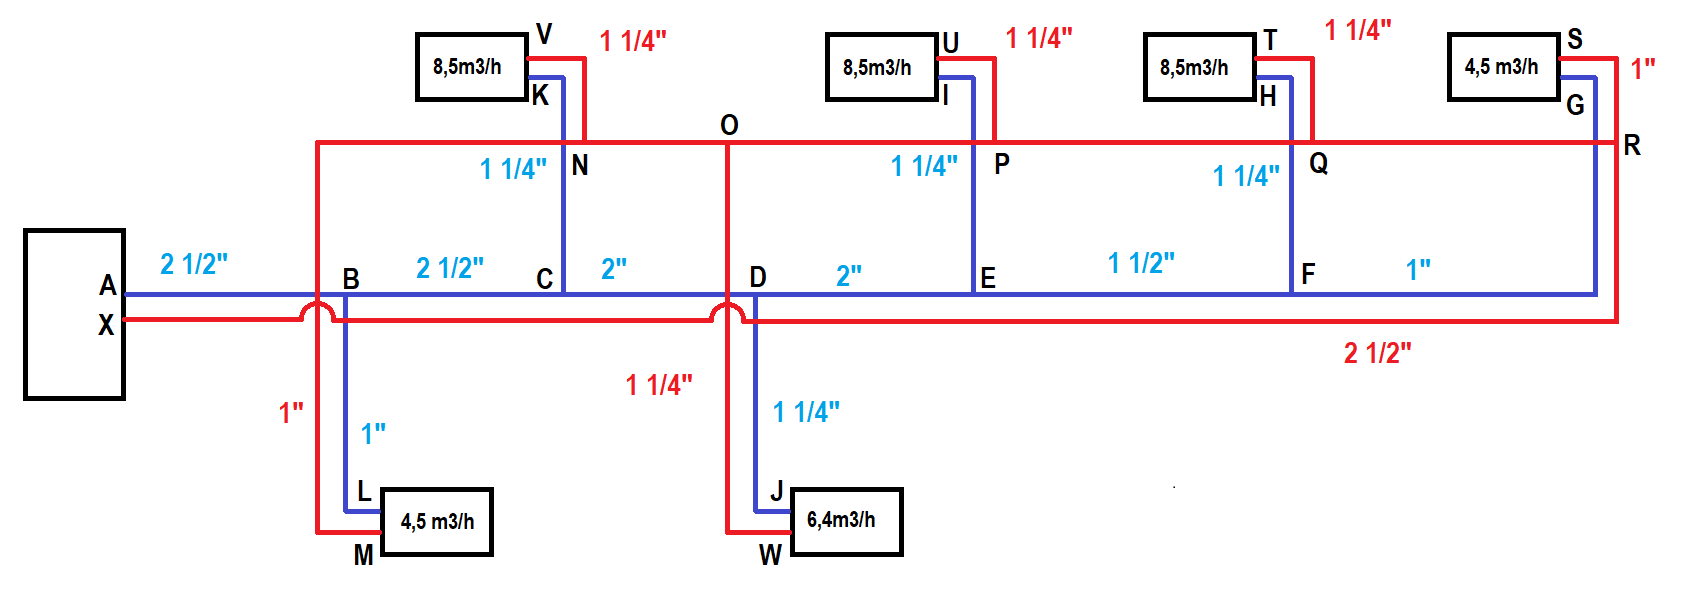
\includegraphics[scale=0.4]{img/o2.png}
\caption{Esquema del sistema de recuperación de calor}
\label{fig:esquema}
\end{figure}

La tabla~\ref{tab:parametros-hidrodinamicos} detalla los parámetros de flujo para cada tramo del sistema, incluyendo caudal, velocidad, largo, diámetro de las tuberías y caída de presión. Estos datos son fundamentales para calcular la eficiencia del sistema y para diseñar la red de tuberías adecuadamente.

\begin{landscape}
\thispagestyle{empty}
\begin{table}[h!]
\centering
\begin{tabularx}{\linewidth}{
  l 
  S[table-format=2.2] 
  S[table-format=1.2] 
  S[table-format=2.2] 
  S[table-format=1.2] 
  S[table-format=1.2] 
  S[table-format=1.2] 
  S[table-format=1.2] 
  S[table-format=3.1] 
  S[table-format=2.1] 
  S[table-format=1.2] 
  S[table-format=1.2]
}
\toprule
\multicolumn{1}{c}{Tramo} & 
\multicolumn{1}{c}{Caudal} & 
\multicolumn{1}{c}{Velocidad} & 
\multicolumn{1}{c}{Largo} & 
\multicolumn{1}{c}{Largo equivalente} & 
\multicolumn{1}{c}{Largo total} & 
\multicolumn{1}{c}{Diámetro} & 
\multicolumn{1}{c}{Caída Presión} & 
\multicolumn{3}{c}{$\Delta P$} \\
\multicolumn{1}{c}{} & 
\multicolumn{1}{c}{(m³/h)} & 
\multicolumn{1}{c}{(m/s)} & 
\multicolumn{1}{c}{(m)} & 
\multicolumn{1}{c}{(m)} & 
\multicolumn{1}{c}{(m)} & 
\multicolumn{1}{c}{(pulg)} & 
\multicolumn{1}{c}{(mmca/m)} & 
\multicolumn{1}{c}{(mmca)} & 
\multicolumn{1}{c}{(Pa)} & 
\multicolumn{1}{c}{(bar)} \\
\midrule
AB & 40,8 & 3,6 & {--} & {--} & {--} & 2~1/2  & 190,3 & {--} & {--} & {--} \\
BC & 36,3 & 3,5 & {--} & {--} & {--} & 2~1/2  & 190,3 & {--} & {--} & {--} \\
CD & 27,8 & 3,3 &      &      &      & 2     & 190,3 &      &      &  \\
DE & 21,4 & 3,1 &      &      &      & 2     & 190,3 &      &      &  \\
EF & 12,9 & 2,6 &      &      &      & 1~1/2 & 190,3 &      &      &  \\
FG & 4,5  & 2   &      &      &      & 1      & 190,3 &      &      &  \\
FH & 8,5  & 2,5 &      &      &      & 1~1/4 & 190,3 &      &      &  \\
EI & 8,5  & 2,5 &      &      &      & 1~1/4 & 190,3 &      &      &  \\
CK & 8,5  & 2,5 &      &      &      & 1~1/4 & 190,3 &      &      &  \\
DJ & 6,4  & 2,4 &      &      &      & 1~1/4 & 190,3 &      &      &  \\
BL & 4,5  & 2   &      &      &      & 1     & 190,3 &      &      &  \\ \midrule
MN & 4,5  & 2   &      &      &      & 1     & 190,3 &      &      &  \\
NO & 12,9 & 2,6 &      &      &      & 1~1/2 & 190,3 &      &      &  \\
OP & 19,4 & 3   &      &      &      & 2     & 190,3 &      &      &  \\
PQ & 27,8 & 3,3 &      &      &      & 2     & 190,3 &      &      &  \\
QR & 36,3 & 3,5 &      &      &      & 2~1/2 & 190,3 &      &      &  \\
RS & 4,5  & 2   &      &      &      & 1     & 190,3 &      &      &  \\
TQ & 8,5  & 2,5 &      &      &      & 1~1/4 & 190,3 &      &      &  \\
UP & 8,5  & 2,5 &      &      &      & 1~1/4 & 190,3 &      &      &  \\
VN & 8,5  & 2,5 &      &      &      & 1~1/4 & 190,3 &      &      &  \\
WO & 6,4  & 2,4 &      &      &      & 1~1/4 & 190,3 &      &      &  \\
RX & 40,8 & 3,6 &      &      &      & 2~1/2 & 190,3 &      &      &  \\
\bottomrule
\end{tabularx}
\caption{Parámetros hidrodinámicos y pérdidas de presión en el sistema de tuberías}
\label{tab:parametros-hidrodinamicos}
\end{table}
\end{landscape}

\subsection{Contexto del Proyecto}
La evolución tecnológica en la industria moderna está conduciendo hacia soluciones que priorizan la eficiencia energética y la sostenibilidad. Una área significativa de oportunidad se encuentra en la planta de producción de Papeles Cordillera S.A., donde se emplean compresores para atender las demandas variadas de aire comprimido, esenciales para los procesos industriales clave. Estos compresores, en su funcionamiento, generan calor residual que, si no es gestionado adecuadamente, puede convertirse en una fuente de pérdida energética y de ineficiencia operacional.\\

La variabilidad inherente en las demandas de los compresores, tal como se indica en la tabla de operaciones (ver Tabla~\ref{tab:compresores_demanda}), subraya la necesidad de un sistema robusto y adaptativo de recuperación de calor. Frente a este escenario, el principal desafío radica en canalizar dicho calor residual, transformándolo en una fuente de energía útil para otros segmentos operativos de la planta. Esta recuperación no solo generaría un beneficio económico tangible, al mitigar los costos energéticos, sino que también posiciona a la empresa como pionera en la adopción de medidas para reducir su huella de carbono.\\

La esencia de este proyecto se centra en dos objetivos fundamentales: eficiencia económica y sostenibilidad. Al potenciar la reutilización del calor y optimizar el perfil de consumo energético, la empresa no solo logra una reducción significativa en gastos operativos, sino que también consolida su posición como referente en la adopción de prácticas industriales ecológicamente responsables.

\subsection{Objetivos Generales y Específicos}

\subsubsection{Objetivo General}
Diseñar un sistema de recuperación de calor eficiente y sostenible derivado del funcionamiento de los compresores en la planta de producción de Papeles Cordillera S.A. Este sistema busca no solo reutilizar el calor residual generado, sino también optimizar el perfil energético global de la planta, conduciendo a una operación más ecológica y económicamente rentable. La meta es convertir una fuente tradicionalmente considerada como pérdida, en un recurso valioso que contribuye a la mejora continua de los procesos industriales y a la reducción del impacto ambiental de la empresa.

\subsubsection{Objetivos Específicos}
\begin{itemize}
\item Evaluación Técnica: Realizar un estudio detallado de las características operativas de los compresores en uso en la planta de Papeles Cordillera S.A., incluyendo las fluctuaciones en demanda, la generación de calor y las condiciones de funcionamiento.
\item Diseño del Sistema: Basado en el análisis previo, diseñar un sistema adaptativo de recuperación de calor que sea capaz de manejar las demandas fluctuantes, seleccionando el tipo de intercambiador de calor más adecuado, ya sea tubular o de placa, y determinando la necesidad de un acumulador de agua.
\item Integración de Infraestructura: Asegurar que el sistema de recuperación de calor esté completamente aislado del sistema de agua industrial de CMPC, garantizando la integridad y calidad de ambos sistemas.
\item Optimización de Flujo: Establecer el sistema de bombeo más eficiente, evaluando la posibilidad de una bomba independiente por equipo o una para el flujo total, y calcular las caídas de presión y diámetros de tuberías adecuados.
\item Análisis de Transferencia Térmica: Calcular la transferencia térmica que se logrará entre el circuito de agua caliente de los compresores y el aporte calórico que se entregará al agua industrial, maximizando la eficiencia en la transmisión de calor.
%\item Evaluación Económica y Ambiental: Realizar un análisis coste-beneficio del sistema propuesto, incluyendo ahorros potenciales en consumo energético y reducción en emisiones de carbono, para validar la rentabilidad y sostenibilidad del proyecto.
%\item {\color{blue} Realizar un análisis termodinámico detallado de las bombas de agua actuales para determinar su eficiencia y relación con el funcionamiento de los compresores}.
%\item Seleccionar bombas de agua que cumplan con los requisitos de rendimiento y eficiencia.
%\item Dimensionar las tuberías del sistema de enfriamiento para garantizar un flujo óptimo y reducir pérdidas.
%\item Seleccionar accesorios y componentes que complementen y mejoren el rendimiento del sistema de enfriamiento.
\end{itemize}


% 5. Descripción del Sistema
\section{Descripción del Sistema}
En Papeles Cordillera S.A., se ha desplegado un sistema de aire comprimido de última generación, diseñado para cumplir con las altas exigencias de sus procesos de producción de manera eficiente y sostenible. Este sistema destaca por su compromiso con la eficiencia energética y la optimización de recursos, evidenciando un enfoque consciente hacia la preservación del medio ambiente.\\

El conjunto de seis compresores de tornillo Kaeser, que constituyen el núcleo del sistema, se distribuyen en tres modelos distintos: tres unidades FSD 575, dos unidades DSDX 305 y una unidad ESD 445. Todos están dotados de un avanzado sistema de recuperación de calor que atrapa y redirige el calor residual de la compresión, facilitando su uso en otras áreas productivas de la planta. Esta integración de tecnología no solo minimiza la pérdida de energía térmica sino que también subraya la ingeniería inteligente del sistema.\\

La eficacia del sistema se ve reforzada por bombas de recirculación estratégicamente instaladas, que garantizan un flujo constante y eficiente del refrigerante entre el acumulador de calor y los intercambiadores, manteniendo así la temperatura óptima del sistema.\\

Para una gestión técnica eficaz, se ha compilado un registro exhaustivo de las especificaciones de cada compresor, que incluye detalles como el modelo, número de serie y potencia nominal, entre otros aspectos vitales. Esta información es crucial para llevar a cabo un mantenimiento preventivo, realizar ajustes precisos y monitorear la eficiencia operativa de manera proactiva.\\


\subsection{Componentes Principales}

\begin{figure}[h]
\centering
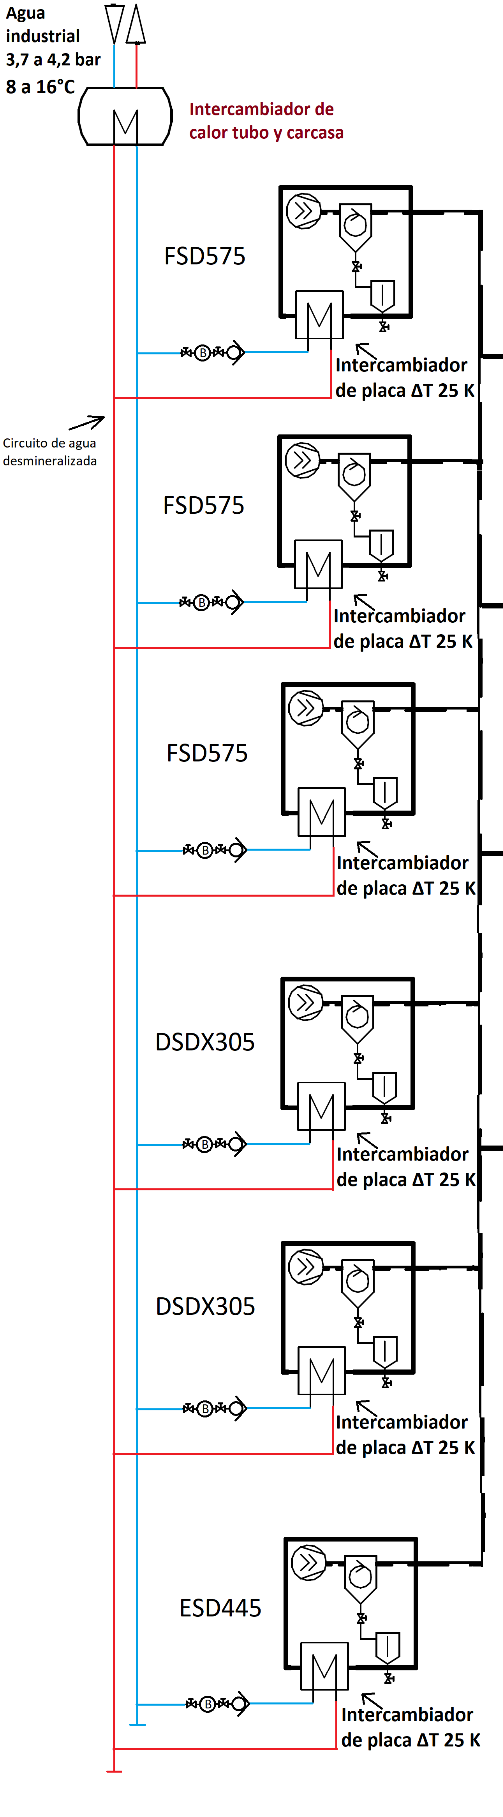
\includegraphics[scale=0.3]{img/esquema.png} % Por supuesto, se debe reemplazar 'sistema.jpg' con el nombre y extensión correctos del archivo de la imagen.
\caption{Esquema del sistema de recuperación de calor propuesto.}
\label{fig:sistema}
\end{figure}

\subsection{Detalles de los compresores de aire}
Los compresores proporcionados por Kaeser Compresores de Chile Spa. a Papeles Cordillera S.A. son unidades de tornillo que emplean dos rotores helicoidales para comprimir el aire. Estos compresores poseen la capacidad de recuperar y reutilizar el calor generado durante el proceso de compresión, lo que resulta en una mejora significativa de la eficiencia energética y la reducción de las emisiones de CO2, aspectos de gran relevancia tanto desde una perspectiva medioambiental como económica. A continuación, se detallan las especificaciones técnicas de estos compresores:

\begin{table}[h]
\footnotesize
\centering
\begin{tabular}{lccc}\toprule
Característica & FSD 575 & DSDX 305 & ESD 445 \\ \midrule
Tipo de compresor & Tornillo de dos etapas & Tornillo de una etapa & Tornillo de dos etapas \\
Numeración & 1, 2, 3 & 4, 5 & 6 \\
Potencia nominal (kW) & 315 & 160 & 250 \\\bottomrule
\end{tabular}
\caption{Especificaciones técnicas de los compresores utilizados en el sistema.}
\label{tab:especificaciones_compresores_ampliadas}
\footnotesize
\textit{Nota:} El compresor FSD 575 (N°3) opera únicamente como respaldo en caso de falla de los compresores N°1 o N°2.
\end{table}

La tabla~\ref{tab:especificaciones_compresores_ampliadas} presenta las especificaciones técnicas de los compresores utilizados en el sistema, incluyendo el nombre del compresor, su número de equipo, la potencia nominal en kilovatios (kW), la presión de descarga en bares (bar), el rendimiento expresado en porcentaje (\%), que indica la eficiencia en la conversión de energía eléctrica en aire comprimido, y el nivel de ruido medido en dB(A). Esta información se basa en la fuente citada \cite{kaeser2023}, que respalda las especificaciones técnicas y ventajas mencionadas anteriormente.


\subsection{Ubicación y Distribución de los Compresores}

En la Figura~\ref{fig:layout_compresores} se presenta un plano que muestra la disposición y ubicación de cada uno de los compresores en la planta de Papeles Cordillera S.A. Se pueden observar cuatro compresores etiquetados del 1 al 4 en la sección derecha del plano, dispuestos verticalmente, y dos compresores adicionales, identificados como 5 y 6, en la sección izquierda. Además, la figura muestra detalles como el sistema de tratamiento de aire, tableros eléctricos y separación de condensado. Esta disposición ha sido diseñada para optimizar la distribución del aire comprimido y para facilitar la intervención y el acceso a cada equipo en caso de necesidad.

\begin{figure}[h]
    \centering
    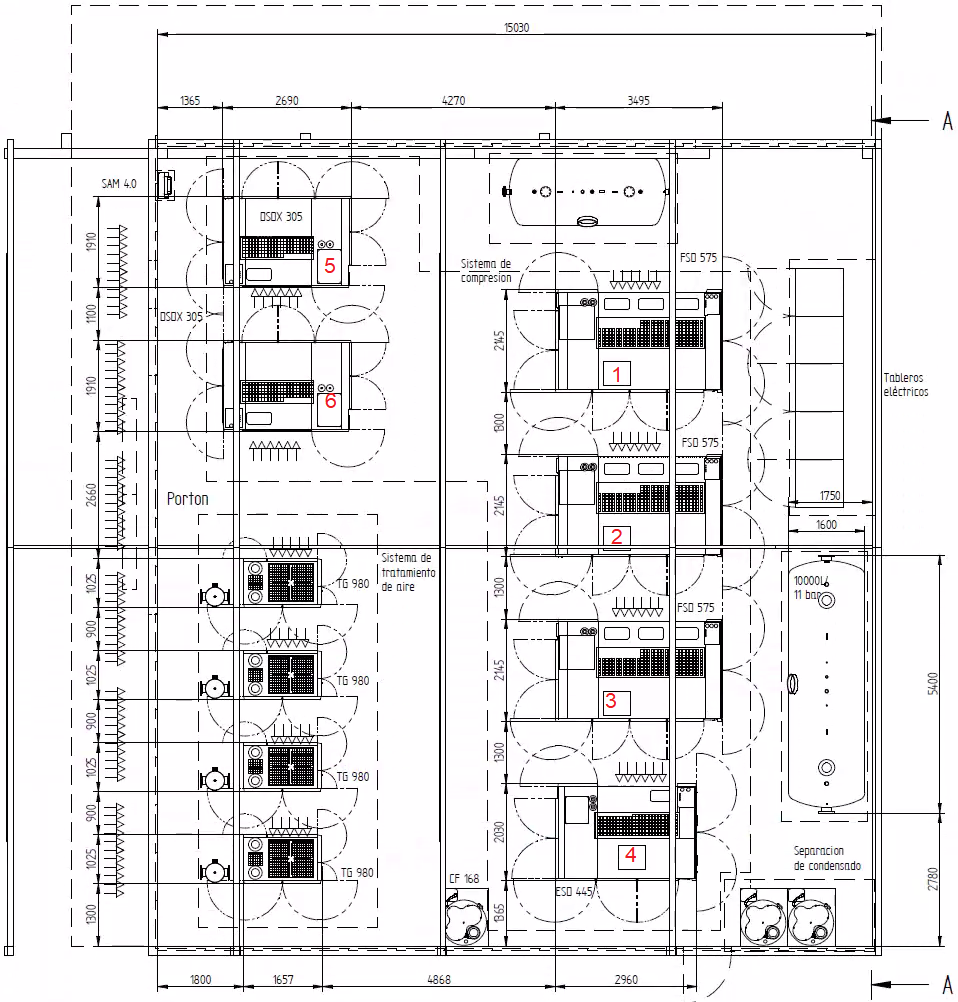
\includegraphics[width=0.8\linewidth]{img/plano_compresores.png}
\caption{Plano de distribución de los compresores en la sala de máquinas.}
    \label{fig:layout_compresores}
\end{figure}

\subsection{Descripción del sistema de enfriamiento}

Los recuperadores de calor son componentes fundamentales en los sistemas de enfriamiento de compresores industriales, desempeñando un papel crucial en la optimización de la eficiencia energética y la reducción de costos operativos en Papeles Cordillera S.A. En esta sección, se presentarán los aspectos técnicos clave de los recuperadores de calor utilizados en los compresores Kaeser, destacando su importancia en el contexto del sistema de enfriamiento. Además, se proporcionará información técnica esencial sobre sus características y capacidades.

\begin{table}[h!]
\footnotesize
\centering
\begin{tabular}{lccc}\toprule
\textbf{Característica} & \textbf{FSD 575} & \textbf{DSDX 305} & \textbf{ESD 445} \\ \midrule
Tipo & Contracorriente & Contracorriente & Contracorriente \\ \hline
\begin{tabular}[c]{@{}l@{}}Eficiencia de recuperación \\ de calor\end{tabular} & Hasta el 90\% & Hasta el 85\% & Hasta el 80\% \\\hline
\begin{tabular}[c]{@{}l@{}}Rendimiento térmico máximo \\ disponible (kW)\end{tabular} & 246 & 130 & 187 \\\hline
\begin{tabular}[c]{@{}l@{}}Agua caliente ($\Delta T=25~\text{K}$) \\ ($\text{m}^3\text{/h}$)\end{tabular} & 8,5 & 4,5 & 6,4 \\\hline
Caída de presión (bar) & 0,4 & 0,25 & 0,4 \\\bottomrule
\end{tabular}
\caption{Información técnica de los recuperadores de calor de los compresores Kaeser.}
\label{tab:recuperador_calor}
\end{table}

La Tabla 1 muestra información técnica relevante sobre los recuperadores de calor de los compresores Kaeser. Estos recuperadores de calor son de tipo contracorriente y pueden alcanzar una eficiencia de recuperación de calor de hasta el $90\%$. El rendimiento térmico máximo disponible es de hasta $246~\text{kW}$, y pueden producir hasta $8,61~\text{m}^3\text{/h}$ de agua caliente con un aumento de temperatura de $25~\text{K}$. Además, la caída de presión en estos recuperadores de calor es de $0,4~\text{bar}$.

\subsection{Especificaciones técnicas de las bombas y tuberías existentes}

El funcionamiento eficiente de la planta industrial de Papeles Cordillera S.A. depende en gran medida de un suministro constante y eficiente de aire comprimido. La Tabla \ref{tab:compresores_demanda} presenta datos cruciales que correlacionan la demanda de aire comprimido con la operación de los compresores, proporcionando información detallada sobre la demanda en metros cúbicos por hora ($\text{m}^3\text{/h}$) y porcentaje, los equipos en funcionamiento, su rendimiento térmico y la producción de agua caliente.

\begin{table}[h]
\footnotesize
\centering
\begin{tabular}{cccccc} \toprule
Grupo & \multicolumn{2}{c}{\begin{tabular}[c]{@{}c@{}}Demanda de aire\\ comprimido\end{tabular}} & \begin{tabular}[c]{@{}c@{}}Equipo en \\ operación\end{tabular} & \begin{tabular}[c]{@{}c@{}}Rendimiento\\ térmico\end{tabular} & \begin{tabular}[c]{@{}c@{}}Agua caliente\\ $\Delta T=25~\text{K}$\end{tabular} \\ 
 & ($\text{m}^3\text{/h}$) & ($\%$) &  & (kW) & ($\text{m}^3\text{/h}$) \\ \midrule
1 & 90 & 2 & 1 - 6 & 442 & 15,32 \\ \midrule
2 & 130 & 1 & 1 - 2 - 4 & 622 & 21,72 \\ \midrule
3 & 131 & 80 & 1 - 2 - 4 & 622 & 21,72 \\ \midrule
4 & 140 & 1 & 1 - 2 - 4 & 622 & 21,72 \\ \midrule
5 & 150 & 1 & 1 - 2 - 6 & 688 & 23,93 \\ \midrule
6 & 174 & 14 & 1 - 2 - 4 - 5 & 752 & 26,22 \\ \midrule
7 & 218 & 2 & 1 - 2 - 4  - 5 - 6 & 948 & 32,93 \\ \bottomrule
\end{tabular}
\caption{Demanda de aire comprimido, rendimiento térmico y producción de agua caliente en grupos de compresores.}
\label{tab:compresores_demanda}
\end{table}

Para garantizar el rendimiento óptimo de los procesos en la planta industrial de Papeles Cordillera S.A., es esencial contar con un suministro constante y eficiente de aire comprimido. Las demandas varían a lo largo de las operaciones diarias, lo que hace imperativo que los compresores e intercambiadores funcionen en sintonía con estas demandas, maximizando la eficiencia y minimizando el desperdicio de recursos. La Tabla \ref{tab:detalles_termicos} resume datos clave, incluyendo la potencia total, el rendimiento térmico máximo y la capacidad para generar agua caliente, proporcionando una visión integral del sistema.

\begin{table}[h]
\footnotesize
\centering
\begin{tabular}{ll} \toprule
\begin{tabular}[c]{@{}l@{}}Potencia total\\ (kW)\end{tabular} & 1.200 \\ \midrule
\begin{tabular}[c]{@{}l@{}}Rendimiento\\ termico max.\\ disponible\\ (kW / MJ/h)\end{tabular} & \begin{tabular}[c]{@{}l@{}}948\\ 3.408\end{tabular} \\ \midrule
\begin{tabular}[c]{@{}l@{}}Agua caliente total\\ $\Delta T=25~\text{K}$\\ ($\text{m}^3\text{/h}$)\end{tabular} & 32,93 \\ \bottomrule
\end{tabular}
\caption{Resumen de potencia total, rendimiento térmico máximo y producción de agua caliente en el sistema.}
\label{tab:detalles_termicos}
\end{table}

Es fundamental comprender estos aspectos del sistema para tomar decisiones informadas y optimizar la operación de la planta.

% 6. Metodología
\section{Metodología}

\subsection{Herramientas y Software Utilizados}

En esta sección, se describen las herramientas y software que se emplearon en el desarrollo del proyecto. La elección de estas herramientas fue fundamental para llevar a cabo un análisis detallado y un diseño preciso del sistema de recuperación de calor en los compresores. Entre las herramientas y software utilizados se incluyen:

\begin{itemize}
    \item Software de simulación termo-fluidodinámica, como [Nombre del Software], para modelar el comportamiento térmico de los compresores y el sistema de enfriamiento.
    \item Hojas de cálculo avanzadas, como Microsoft Excel, para realizar cálculos detallados de transferencia de calor y dimensionamiento de componentes.
    \item Herramientas de diseño asistido por computadora (CAD), como [Nombre del Software CAD], para la creación de planos y diseños de componentes del sistema.
\end{itemize}

\subsection{Procedimientos y Técnicas de Cálculo}

En el estudio y diseño de un sistema de enfriamiento para el compresor, es esencial comprender y aplicar adecuadamente las ecuaciones de transferencia de calor. Estos principios son fundamentales para el manejo del exceso de temperatura generado por el compresor y son una parte crucial de la metodología utilizada en este proyecto. A continuación, se describen los principios básicos de transferencia de calor relevantes:

\subsubsection{Principios Básicos de Transferencia de Calor en el Compresor}

El calor tiende a fluir desde regiones de mayor temperatura a regiones de menor temperatura. Por lo tanto, para enfriar eficazmente el compresor, se utiliza un medio de enfriamiento, como agua, que esté a una temperatura más baja que la temperatura generada por el compresor. La diferencia entre estas dos temperaturas se conoce como $\Delta T$ del sistema.

\subsubsection{Ecuaciones de Transferencia de Calor Relevantes}

A lo largo de este proyecto, se aplicaron diversas ecuaciones de transferencia de calor para analizar y diseñar el sistema de recuperación de calor en los compresores. Algunas de las ecuaciones clave utilizadas incluyen:

\begin{enumerate}
    \item \textbf{Transferencia de calor por conducción}: La transferencia de calor por conducción a través de sólidos es un fenómeno clave en la ingeniería de transferencia de calor y es fundamental para el diseño de intercambiadores de calor. Esta se rige por la Ley de Conducción de Fourier \cite{incropera2002}:

\begin{align}
Q = -k \cdot A \cdot \frac{dT}{dx}
\label{eq:conduccion}
\end{align}

Donde:
\begin{itemize}
    \item $Q$ es la tasa de transferencia de calor.
    \item $k$ es la conductividad térmica del material.
    \item $A$ es el área de sección transversal a través de la cual se produce la transferencia de calor.
    \item $dT/dx$ es el gradiente de temperatura en la dirección de transferencia de calor.
\end{itemize}

%Como se describe en \cite{incropera2002}, p. 145.

    \item \textbf{Transferencia de calor por cambio de entalpía}:La transferencia de calor por cambio de entalpía es relevante para describir el cambio de calor en procesos adiabáticos. Se expresa mediante la ecuación \cite{cengel2014}:

\begin{align}
Q = \Delta h \cdot m
\label{eq:entalpia}
\end{align}

Donde:
\begin{itemize}
    \item $Q$ es la cantidad de calor transferido.
    \item $\Delta h$ es el cambio de entalpía.
    \item $m$ es la tasa de flujo de masa del fluido.
\end{itemize}

%Como se describe en \cite{cengel2014}, p. 352.

    \item \textbf{Transferencia de calor por convección}: La transferencia de calor por convección describe el transporte de calor entre una superficie sólida y un fluido circundante y se basa en la Ley de Enfriamiento de Newton \cite{incropera2002}:

\begin{align}
Q = h \cdot A \cdot \Delta T
\label{eq:conveccion}
\end{align}

Donde:
\begin{itemize}
    \item $Q$ es la tasa de transferencia de calor.
    \item $h$ es el coeficiente de transferencia de calor por convección.
    \item $A$ es el área de superficie a través de la cual se produce la transferencia de calor.
    \item $\Delta T$ es la diferencia de temperatura entre la superficie y el fluido.
\end{itemize}
%Como se describe en \cite{incropera2002}, p. 226.

\end{enumerate}

Estas ecuaciones fundamentales proporcionan la base para comprender y analizar la transferencia de calor en sistemas de enfriamiento de compresores. Dependerá de las condiciones específicas del sistema y los parámetros elegidos cuál de estas ecuaciones es más aplicable en un contexto dado.

\begin{table}[h]
\centering
\resizebox{\textwidth}{!}{%
\begin{tabular}{|c|c|c|}
\hline
\textbf{Constante Térmica} & \textbf{Posibles Valores (SI)} & \textbf{Comentarios} \\ \hline
Conductividad Térmica ($k$) & Acero inoxidable: 16-19 W/(m·K) & Dependiente del material \\ \hline
Coeficiente de Transferencia de Calor ($h$) & Aire (natural): 5-25 W/(m²·K) & Varía con la velocidad del flujo \\ \hline
Área de Superficie ($A$) & Variable & Depende de la geometría \\ \hline
Gradiente de Temperatura ($\frac{dT}{dx}$) & Variable & Depende de las condiciones \\ \hline
Cambio de Entalpía ($\Delta h$) & Variable & Depende del fluido y condiciones \\ \hline
Tasa de Flujo de Masa ($m$) & Variable & Depende de la demanda de enfriamiento \\ \hline
Diferencia de Temperatura ($\Delta T$) & Variable & Depende de las temperaturas \\ \hline
\end{tabular}%
}
\caption{Posibles valores de constantes térmicas en el contexto del sistema de enfriamiento del compresor.}
\label{tab:constantes_termicas}
\end{table}
\subsection{Aplicación al Compresor}

Para el compresor en cuestión, estas ecuaciones permitieron calcular la cantidad de calor que se debe eliminar, el medio de enfriamiento adecuado, el tamaño y especificaciones del intercambiador de calor, entre otros detalles técnicos. Las ecuaciones también proporcionaron información sobre cómo optimizar el sistema para garantizar una operación eficiente y segura del compresor.

% 7. Resultados
\section{Resultados}

\subsection{Memoria de Cálculo y Análisis Termodinámico}
Detalles de los cálculos realizados.

Análisis termodinámico y sus implicaciones.

\subsection{Selección de Bombas}
Opciones consideradas.

Justificación de la elección.

\subsection{Dimensionamiento de Tuberías}
Cálculos y criterios utilizados.

Recomendaciones para la instalación.

\subsection{Selección de Accesorios y Componentes Adicionales}
Lista de componentes seleccionados.

Justificación y especificaciones técnicas.


\subsection{Recuperación de Calor de Compresores}
Primero, vamos a calcular la cantidad de calor que se puede recuperar de los grupos de compresores en operación. Utilizaremos la fórmula:

\begin{align*}
\text{Calor recuperado (kW)} &= \text{Demanda de aire comprimido} \times \text{Rendimiento térmico} \times \frac{\%}{100}
\end{align*}

donde:
\begin{itemize}
    \item \textit{Demanda de aire comprimido} se encuentra en la columna correspondiente en la Tabla 1.
    \item \textit{Rendimiento térmico} se encuentra en la columna correspondiente en la Tabla 1.
    \item $\%$ se encuentra en la columna correspondiente en la Tabla 1 y se refiere al porcentaje de tiempo en que opera cada equipo.
\end{itemize}

Luego, calcularemos la cantidad de agua caliente que se puede producir en base a la cantidad de calor recuperado. Usaremos la fórmula:

\begin{align*}
\text{Agua caliente producida ($\text{m}^3\text{/s}$)} &= \frac{\text{Calor recuperado (kW)}}{\text{Rendimiento térmico disponible (kW)}}
\end{align*}

donde \textit{Rendimiento térmico disponible} se encuentra en la tabla proporcionada anteriormente.\\

 En la Tabla~\ref{tab:calor_agua_caliente}, se presenta un resumen del calor recuperado y la cantidad de agua caliente producida por los compresores en operación. Los grupos de compresores se enumeran en la columna ``Grupo'', y los equipos específicos que operan en cada grupo se detallan en la columna ``Equipos''. El ``Calor'' se expresa en kilovatios (kW), y la ``Agua caliente producida'' se mide en metros cúbicos por hora ($\text{m}^3\text{/h}$).\\


\begin{table}[h]
\footnotesize
\centering
\begin{tabular}{cccccccc} \toprule
Grupo & \multicolumn{1}{c}{\begin{tabular}[c]{@{}c@{}}Equipo en \\ operación\end{tabular}} & \begin{tabular}[c]{@{}c@{}}Calor recuperado\\ \end{tabular} & \begin{tabular}[c]{@{}c@{}}Agua caliente producida\\ \end{tabular} \\ 
 &  & (kW) & ($\text{m}^3\text{/h}$) \\ \midrule
1 & 1 - 6 & 795,6 & 1,8 \\ \midrule
2 & 1 - 2 - 4 & 808,6 & 1,3 \\ \midrule
3 & 1 - 2 - 4 & 65.185,6 & 104,8 \\ \midrule
4 & 1 - 2 - 4 & 870,8 & 1,4 \\ \midrule
5 & 1 - 2 - 6 & 1032 & 1,5 \\ \midrule
6 & 1 - 2 - 4 - 5 & 18.318,72 & 24,36 \\ \midrule
7 & 1 - 2 - 4 - 5 - 6 & 4.133,28 & 4,36 \\ \bottomrule
\end{tabular}
\caption{Resumen del calor recuperado y agua caliente producida por los compresores en operación.}
\label{tab:calor_agua_caliente}
\end{table}

Con estos cálculos, obtenemos la cantidad de calor recuperado y la cantidad de agua caliente producida por los compresores en operación. Estos datos son importantes para evaluar la eficiencia del sistema y la capacidad de recuperación de calor.

% 8. Conclusiones
\section{Conclusiones}
Resumen de los hallazgos clave.

Beneficios esperados de las recomendaciones propuestas.

% 9. Recomendaciones
\section{Recomendaciones}
Sugerencias para la implementación.

Mantenimiento y cuidados a considerar.

% 10. Anexos
\appendix
\section{Anexos}
Cualquier dato adicional, gráficos, tablas, etc.

Copias de cálculos detallados o software utilizado.

% 11. Referencias
\bibliographystyle{unsrt} % O el estilo que prefieras.
\bibliography{referencias.bib} % Asume que tienes un archivo 'referencias.bib' con tus citas.

\clearpage

\end{document}
